% small.tex
\documentclass{beamer}
\usetheme{Boadilla}
\setbeamertemplate{blocks}[rounded][shadow=false] 

\usepackage{subfig}
\usepackage{multirow}
\usepackage{amsmath}
\usepackage{mathtools}
\usepackage{listings}
\usepackage{color}
 
\definecolor{dkgreen}{rgb}{0,0.6,0}
\definecolor{gray}{rgb}{0.5,0.5,0.5}
\definecolor{mauve}{rgb}{0.58,0,0.82}

\lstset{ %
  language=Python,                % the language of the code
  basicstyle=\footnotesize,           % the size of the fonts that are used for the code
  %numbers=left,                   % where to put the line-numbers
  %numberstyle=\tiny\color{gray},  % the style that is used for the line-numbers
  %stepnumber=2,                   % the step between two line-numbers. If it's 1, each line 
                                  % will be numbered
  %numbersep=5pt,                  % how far the line-numbers are from the code
  %backgroundcolor=\color{white},      % choose the background color. You must add \usepackage{color}
  showspaces=false,               % show spaces adding particular underscores
  showstringspaces=false,         % underline spaces within strings
  showtabs=false,                 % show tabs within strings adding particular underscores
  %frame=single,                   % adds a frame around the code
  rulecolor=\color{black},        % if not set, the frame-color may be changed on line-breaks within not-black text (e.g. commens (green here))
  tabsize=2,                      % sets default tabsize to 2 spaces
  captionpos=b,                   % sets the caption-position to bottom
  breaklines=true,                % sets automatic line breaking
  breakatwhitespace=false,        % sets if automatic breaks should only happen at whitespace
  title=\lstname,                   % show the filename of files included with \lstinputlisting;
                                  % also try caption instead of title
  keywordstyle=\color{blue},          % keyword style
  commentstyle=\color{dkgreen},       % comment style
  stringstyle=\color{mauve},         % string literal style
  escapeinside={\%*}{*)},            % if you want to add a comment within your code
  morekeywords={dynamic, string}               % if you want to add more keywords to the set
}


\AtBeginSection[]
{
  \begin{frame}
    \frametitle{Table of Contents}
    \tableofcontents[currentsection]
  \end{frame}
}


%About me
\author{Wesley Brooks} 
\title[Varying-coefficients selection]{Selection and estimation for varying-coefficients regression}
%\subtitle{sub} 
\institute{UW-Madison} 

\begin{document}

%Title slide
\begin{frame}
\titlepage
\end{frame}


%Table of contents
\begin{frame}{Outline}
  \tableofcontents
\end{frame}




\section{Varying-coefficients regression}

\begin{frame}{Varying-coefficients regression}
\begin{itemize}
	\item What if the effect of my variable is not constant?
	\begin{itemize}
		\item Agriculture more valuable in regions with richer soil
		\item Mining more valuable in regions with greater mineral deposits
	\end{itemize}
	\item Consider coefficients as functions of location: $\beta(s)$
	\item How to estimate $\beta(s)$?
\end{itemize}
\end{frame}


\begin{frame}{Estimating coefficient functions}
\begin{itemize}
	\item Estimate model locally at each model point
	\begin{itemize}
		\item Give weight to each observation based on distance from model point
		\item Multiply design matrix by weight matrix
		\item Use the adaptive Lasso for selection/estimation
	\end{itemize}
\end{itemize}

\begin{figure}
\begin{center}
	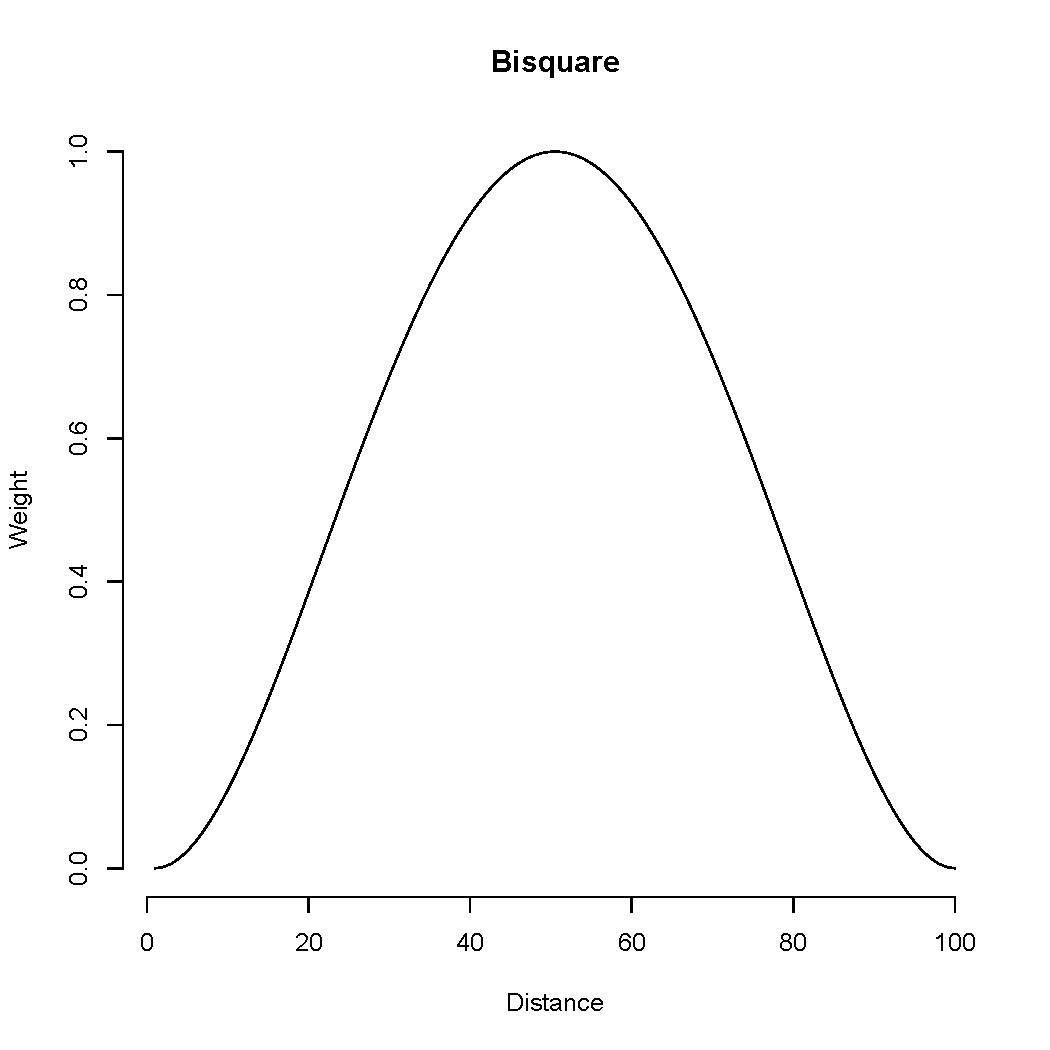
\includegraphics[width=0.4\textwidth]{../../figures/simulation/illustrations/bisquare}
	\caption{The bisquare kernel.}
\end{center}
\end{figure}

\end{frame}


\begin{frame}{Model parameter selection}
Estimate model parameters using the AIC
\begin{itemize}
	\item Each model point has a Lasso tuning parameter
	\begin{itemize}
		\item Use local AIC
	\end{itemize}
	
	\item Bandwidth for the kernel function
	\begin{itemize}
		\item Use total AIC
	\end{itemize}
\end{itemize}
\end{frame}


\section{Simulation study}

\begin{frame}{Simulation study} 

\begin{itemize}
	\item Five covariates simulated on a $30 \times 30$ grid with a GRF
	\item True coefficient surfaces: $\beta_1$ below, $\beta_2$ - $\beta_5 \equiv 0$ everywhere
	\item Random error simulated from a GRF
	\begin{itemize}
		\item $\rho:$ between-covariates correlation ($0, 0.5, 0.8$)
		\item $\tau_x:$ spatial autocorrelation of the covariates ($0.03, 0.1$)
		\item $\tau_\sigma:$ spatial autocorrelation of the random errors ($0, 0.03, 0.1$)
	\end{itemize}
\end{itemize}
\vspace{-4mm}
\begin{figure}
\begin{center}
	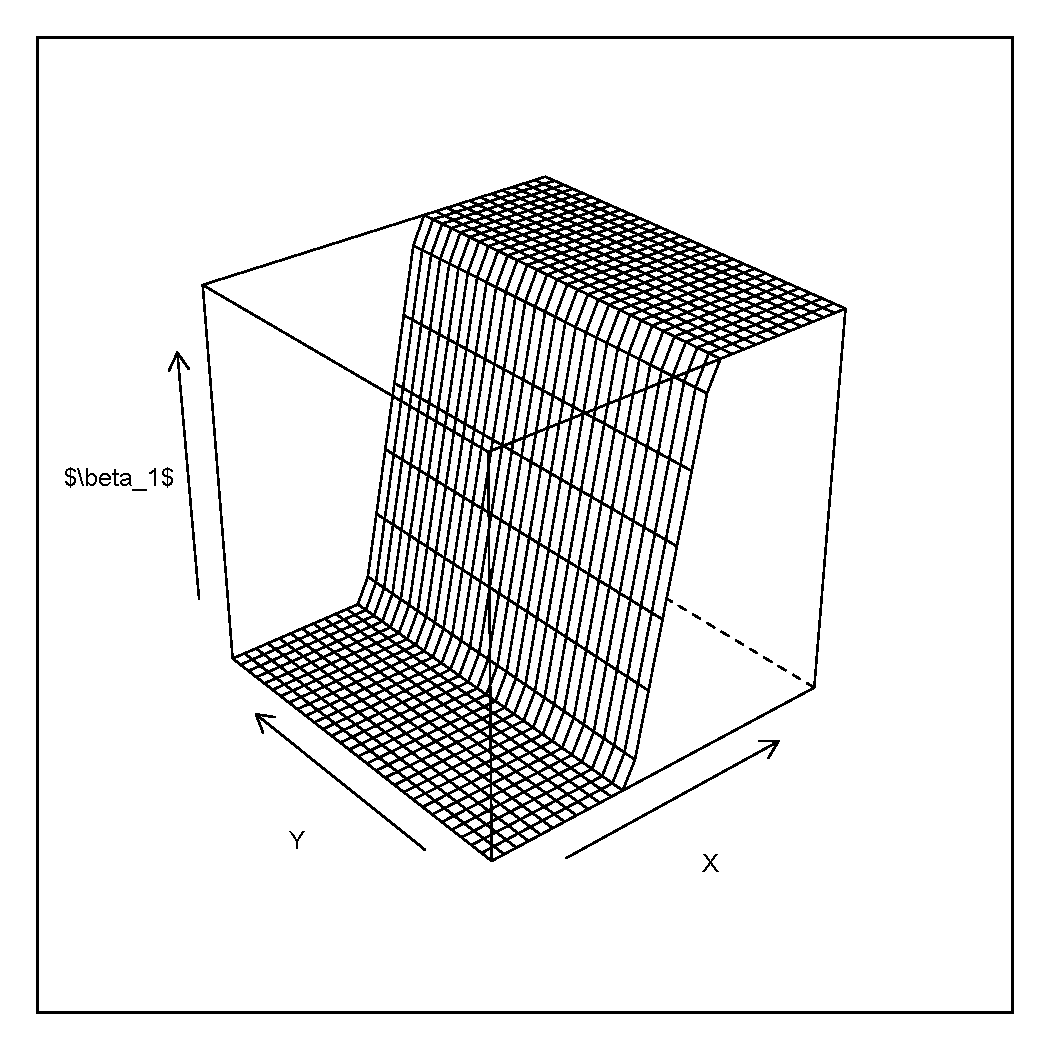
\includegraphics[width=0.4\textwidth]{../../figures/simulation/illustrations/beta1-actual}
	\caption{The true coefficient surface for $\beta_1$.}
\end{center}
\end{figure}
\end{frame} 

\begin{frame}{Simulation result - estimate of $\beta_1$} 

\begin{itemize}
	\item Simulation setting: $\rho=0$, $\tau_x=0.03$, $\tau_\sigma=0$
\end{itemize}
\vspace{-10mm}
\begin{figure}
\begin{center}
	\subfloat[]{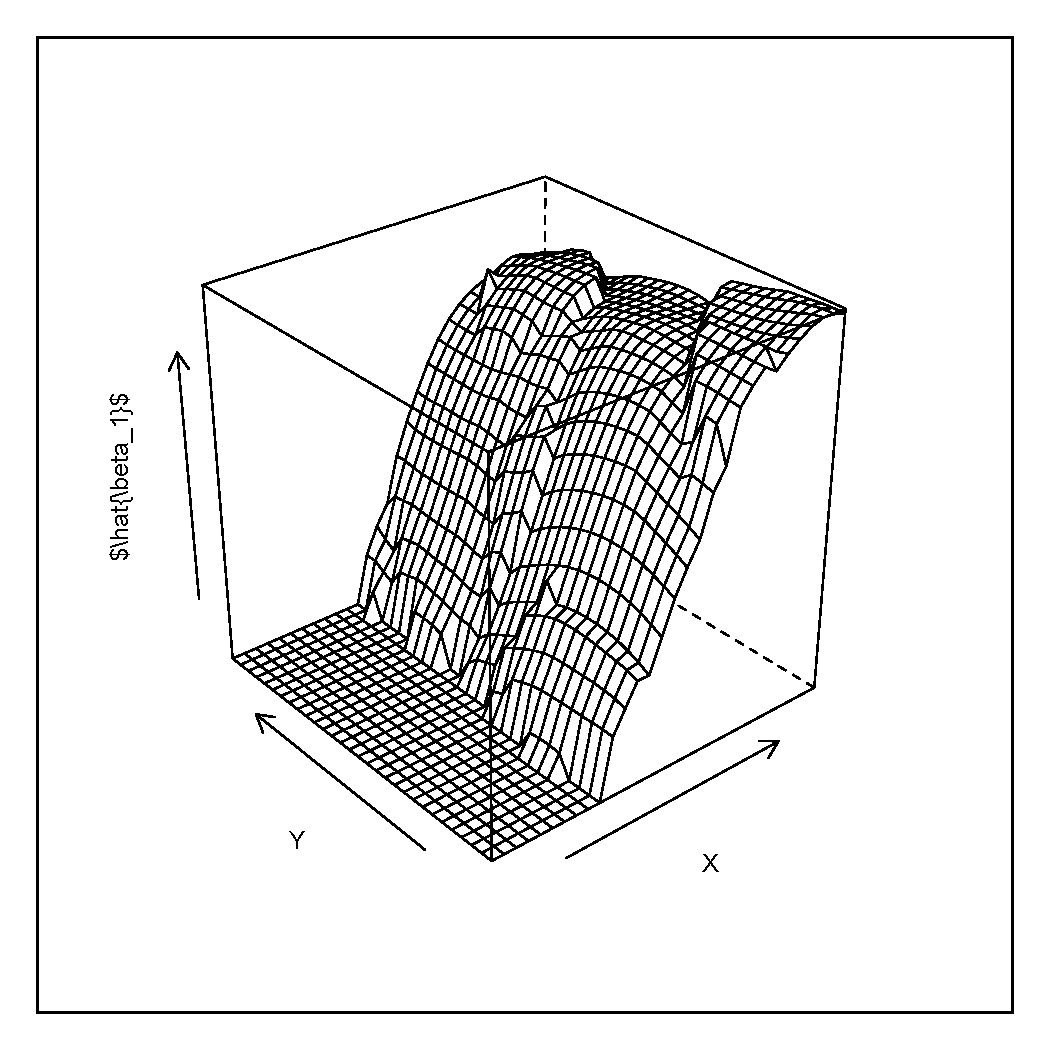
\includegraphics[width=0.45\textwidth]{../../figures/simulation/illustrations/setting1-beta1-estimate}}
	\subfloat[]{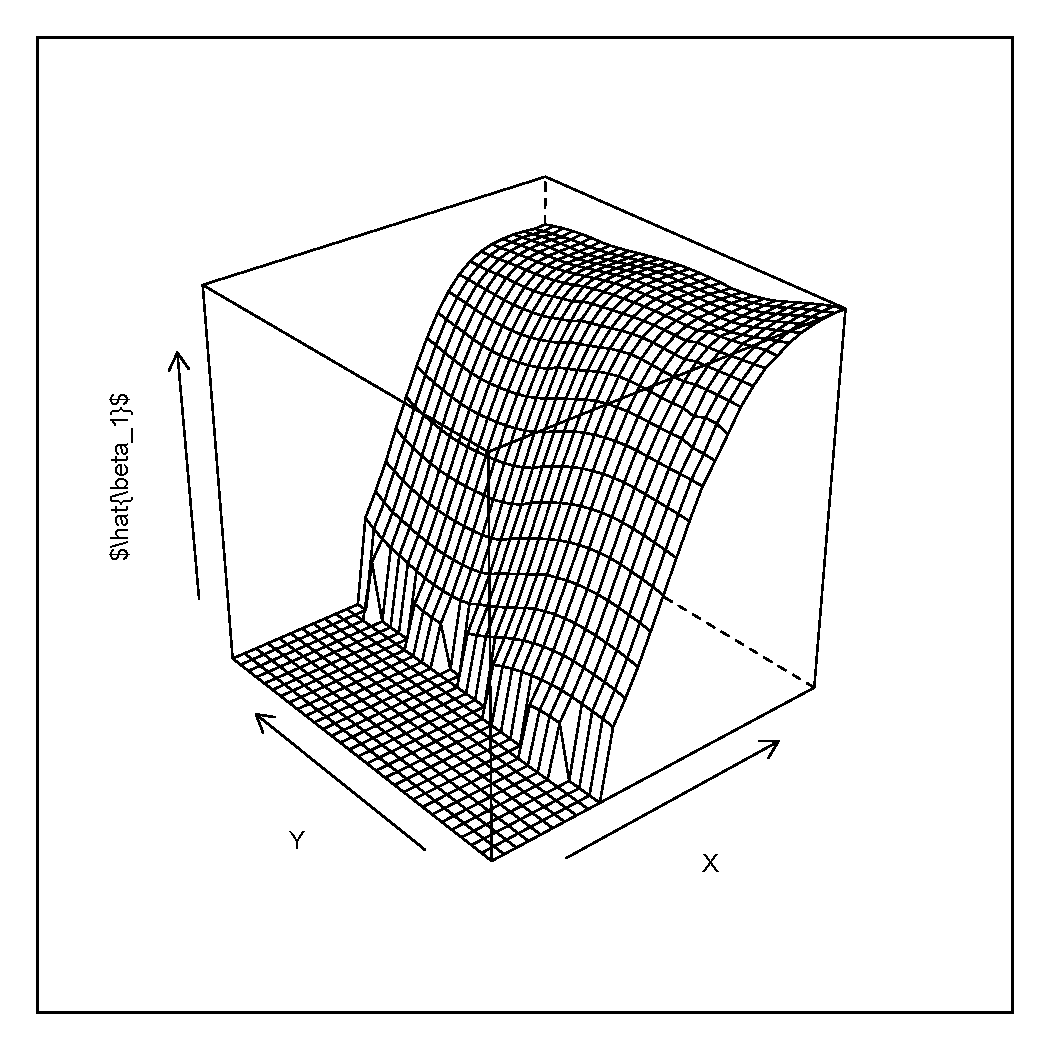
\includegraphics[width=0.45\textwidth]{../../figures/simulation/illustrations/setting1-beta1-estimate-unshrunk}}
	\caption{Left: estimated using GWL for selection and estimation; Right: GWL for selection, least squares for estimation.}
\end{center}
\end{figure}
\end{frame} 

\begin{frame}{Simulation result - estimate of $\beta_1$} 

\begin{itemize}
	\item Simulation setting: $\rho=0.8$, $\tau_x=0.1$, $\tau_\sigma=0.1$
\end{itemize}
\vspace{-10mm}
\begin{figure}
\begin{center}
	\subfloat[]{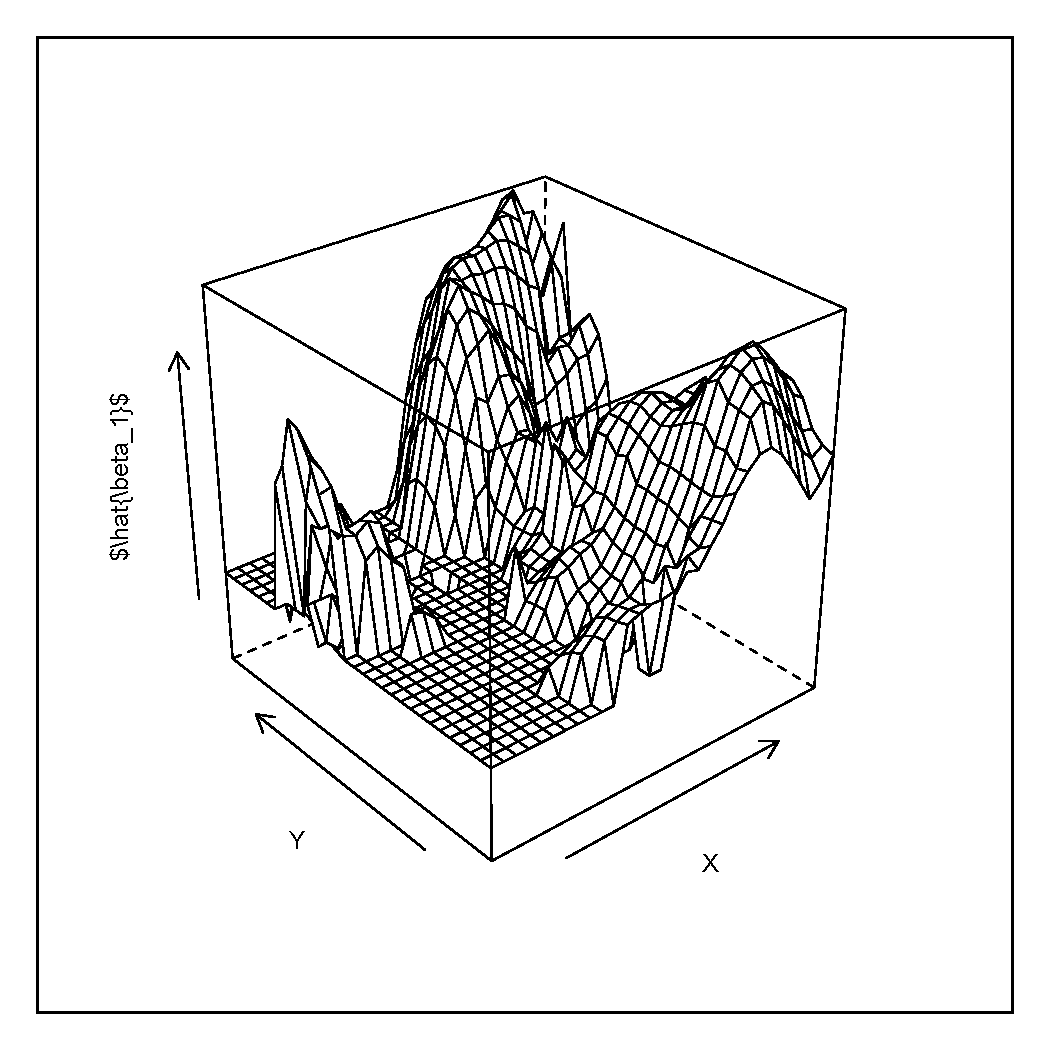
\includegraphics[width=0.45\textwidth]{../../figures/simulation/illustrations/setting18-beta1-estimate}}
	\subfloat[]{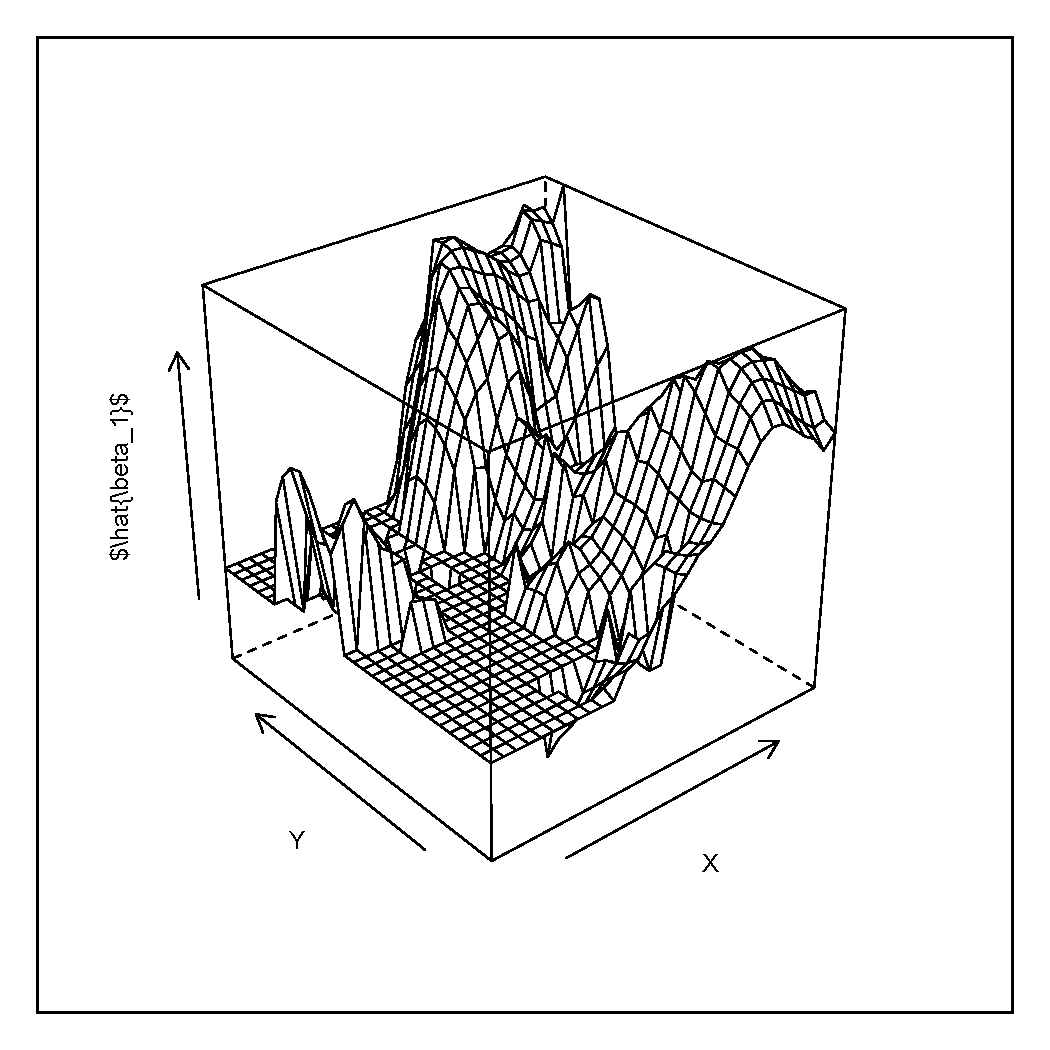
\includegraphics[width=0.45\textwidth]{../../figures/simulation/illustrations/setting18-beta1-estimate-unshrunk}}
	\caption{Left: estimated using GWL for selection and estimation; Right: GWL for selection, least squares for estimation.}
\end{center}
\end{figure}
\end{frame} 


\section{Census data}


\begin{frame}{Census data: model of poverty rate} 
Images are separate
\end{frame} 


\end{document}
